\chapter{Mitigate Fingerprint Activities of Honeypots}
\label{chap:fingerprinting}

\epigraph{There is a generic weakness in the current generation of low- and medium-interaction honeypots because of their reliance on off-the-shelf libraries to implement large parts of the transport layer.}{\textit{Alexander Vetterl}}

Detecting honeypots before launching attacks helps to avoid disclosure of information.
In \autoref{chap:cloud-security}, we have seen that bot activities are on the rise, and more attacks than ever have been launched.
However, the vast majority of attacks have been identified to be repetitive.
In this chapter, we will conduct two experiments related to the question if it is possible to fingerprint honeypots.
First, we want to reproduce the findings that \citet{vetterl2020} claims to prove the initial question if any fingerprint activity is feasible.
Lastly, we present a concept to disguise Cowrie, and verfiy our assumption with an experiment.

\section{OpenSSH}
\label{sec:openssh}

OpenSSH is one of the most used applications that enables SSH.
Before proceeding with generic weaknesses of honeypots, we want to give a short intermezzo about OpenSSH itself.

\begin{figure}
    \centering
    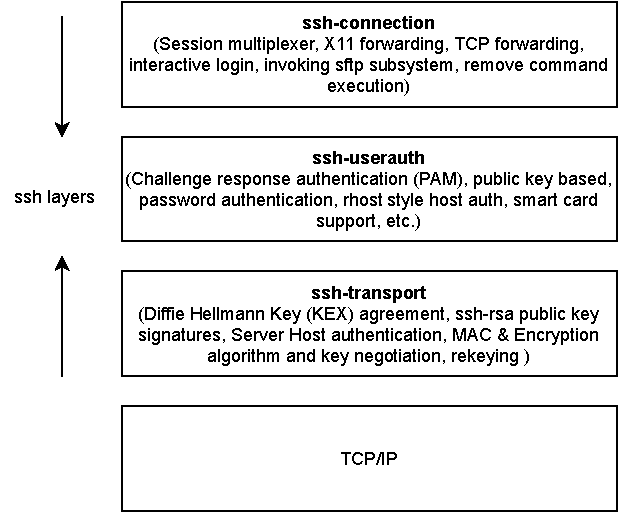
\includegraphics{figures/openssh-architecture.pdf}
    \caption[OpenSSH architecture]{OpenSSH architecture (derived from \cite{openssh2007})}
    \label{fig:openssh-architecture}
\end{figure}

OpenSSH consists of three major layers, namely \verb|ssh-connection|, \verb|ssh-userauth|, and \verb|ssh-transport| (\autoref{fig:openssh-architecture}).
Last layer is the most important one because it provides the basic functionalities for crypto operations such as the key exchange and encryption.

The first layer is responsible for authenticating the user to the sshd daemon.
Based on two-way authentication, the client authenticates the sshd daemon by the help of the \verb|ssh-transport|.
Finally, a secure connection is established, and the key exchange is done.
Next step is to authenticate the user of the client.
It offers various authentication methods such as username/password, public key, or smart-card authentication.
If the \verb|ssh-userauth| layer is successful, it will establish a secure channel through the \verb|ssh-connection| layer.
Each session is handled in a so-called channel.

The \verb|ssh-connection| layer handles multiple sessions simultaneously over a single \verb|ssh-userauth| layer with the TCP/IP layer below.
It is responsible for executing arbitrary commands, forwarding X11 connections, establishing VPN tunnels and more.

In addition, OpenSSH comes with built-in features such as keep alive messages, redirecting stdin to /dev/null for specialized X11 windows.

\autoref{fig:openssh-flow-diagram} outlines a sample session between a client and a server.
The key exchange initialization is the first message between them to negotiate all ciphers and keys for communication.
For this chapter, no other than this message will be considered.

\section{Preliminary Work}

Attackers have a strong motivation to reveal honeypots before launching an attack.
Without any protection attackers would disclose their methods, and thus, newly developed attacks would become useless.
As shown in \autoref{chap:cloud-security}, attackers do try to get information about the host system.
\citet{vetterl2020} discussed various methods of fingerprinting, however, executing commands in a shell and examining the response leaves precarious information to the honeypot itself.
In his work he evaluated methods to detect honeypots at the transport level.
As stated, the value of a honeypot would be merely zero if a detection on transport level would work.
He presents fingerprinting methods for SSH, Telnet, and HTTP/Web.
Due to the complexity of each method, we focus on SSH fingerprinting with the honeypot Cowrie.
The idea to detect SSH honeypots is to look for deviations in the response.
Therefore, \citet{vetterl2020} sends a set of probes $P = \{P_1, P_2, \dots, P_n\}$ to a given set of implementations of a network protocol $I = \{I_1, I_2, \dots, I_n\}$ and stores the set of responses $R = \{R_1, R_2, \dots, R_n\}$.
For the given set of responses he calculated the cosine similarity coefficient $C$.
Goal is to find the best $P_i$ where the sum of $C$ is the lowest.
\autoref{fig:draft-cosine-similarity} presents these steps.

Cosine similarity outputs the similarity between vectors of numerical attributes.
It is widely used in text semantics to measure the similarity of sets of information such as two sentences.
\citet{vetterl2020} outlines that it can be used in \enquote{traffic analysis to find abnormalities and to measure domain similarity}.
Mathematically, it computes the angle between two vectors.
For each set of information $A$, we create a vector $D_A$.
Referring to our use case with SSH, we use the response from the server as information $A$.
If $\theta$ is the angle between $D_A$ and $D_B$, then:

\begin{equation} \label{eq:cosine-similarity}
    \cos \theta = \frac{D_A \cdot D_B}{\|D_A\| \|D_B\|}
\end{equation}

where \enquote{$\cdot$} is the dot product obtained by:

\begin{equation}
    D_A \cdot D_B = \sum_{i=1}^{n} (D_{A_i} \times D_{B_i})
\end{equation}

and $\|D_A\|$ (resp. $\|D_B\|$) is the Euclidean norm, obtained by $\sqrt{\sum_{i=1}^{n} D_{A_i}^2}$ (resp. $\sqrt{\sum_{i=1}^{n} D_{B_i}^2}$).
The values of vectors are non-negative. The similarity between items is the value $\cos \theta$, $\cos \theta = 1$ indicates equality.

\begin{figure}[ht]
    \centering
    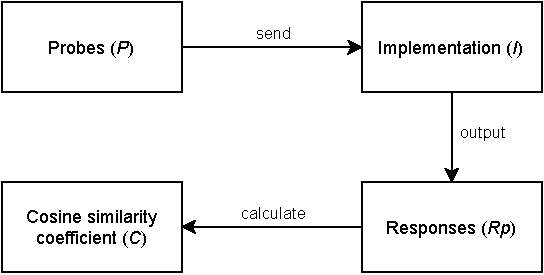
\includegraphics{figures/vetterl_concept.pdf}
    \caption[Outline to obtain the cosine similarity coefficient]{Outline to obtain the cosine similarity coefficient (derived from \cite{vetterl2020}).}
    \label{fig:draft-cosine-similarity}
\end{figure}

In order to find the best $P_i$ for SSH, \citet{vetterl2020} first created different SSH version strings based on the format: \verb|SSH-protoversion-swversion SP comment crlf|.
He used different lower and upper case variations, 12 different protoversions ranging from $0.0$ to $3.2$, swversion set to \enquote{OpenSSH} or empty string, comment set to \enquote{FreeBSD} or empty string, and crlf to either \verb|\r\n| or empty string.
In total, summing up to 192 client version strings.
Second, he created different \verb|SSH2_MSG_KEXINIT| packets with 16 key-exchange algorithms, 2 host key algorithms, 15 encryption algorithms, 5 MAC algorithms and 3 compression algorithms.
In total, he sent \numprint{58752} \verb|SSH2_MSG_KEXINIT| packets.
Combining them with the 192 client versions, he ended up sending \numprint{157925376} packets.
The version string \verb|SSH-2.2-OpenSSH \r\n| and the \verb|SSH2_MSG_KEXINIT| packet including ecdh-sha2-nistp521 as key-exchange algorithm, ssh-dss as host key algorithm, blowfish-cbc as encryption algorithm, hmac-sha1 as mac algorithm and zlib@openssh.com as compression algorithm, with the wrong padding result in the lowest cosine similarity coefficient $C$.
\autoref{lst:ssh-debug} shows the SSH debug information with the modified version string, and key exchange message.

\begin{figure}
    \lstinputlisting[language=bash, caption={[Example OpenSSH connection with probed SSH packet]OpenSSH connection attempt with probed SSH packet. All non-essential debug information have been removed to lay emphasis on the modified key exchange initialization.}, label={lst:ssh-debug}]{listings/ssh-debug.txt}
\end{figure}

\autoref{tab:cosine-similarity} has been derived from \citet{vetterl2020} to present his results of the cosine similarity of OpenSSH, Twisted, and Cowrie.
Twisted has been added to have an example with an older SSH honeypot.
We can see that it differs fundamentally from OpenSSH.
At most, it scores $0.52$ whereas various OpenSSH versions start at $0.98$.
The number of hosts significantly decreases with a cosine similarity score of $0.90$ and higher.
Cowrie responses are not too far away to OpenSSH with an average of $0.80$.
However, scanning through the web with a minimum score of $0.90$ and higher would exclude all honeypots.
Thus, distinguishing Cowrie from OpenSSH with SSH packets is a feasible method.
Moreover, \citet{vetterl2020} performed an Internet-wide scan, and detected $758$ Kippo and $2021$ Cowrie honeypots.
These results show that the values of honeypots would decrease to zero when large fingerprinting activities are used.

\begin{figure}[ht]
    \centering
    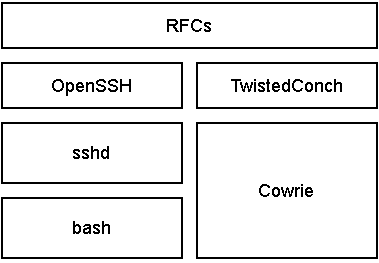
\includegraphics{figures/cowrie-openssh.pdf}
    \caption[Architecture of OpenSSH and Cowrie]{Architecture of OpenSSH and Cowrie. OpenSSH and TwistedConch have subtle differences (derived from \cite{vetterl2020})}
    \label{fig:cowrie-openssh}
\end{figure}

\citet{vetterl2020} states that current low- and medium-interaction honeypots have a generic weakness due to the underlying off-the-shelf libraries.
Cowrie is based on TwistedConch\footnote{\href{https://github.com/racker/python-twisted-conch/commit/01f22a3a8534856e934ed716cfc251b04e7d2077}{TwistedConch 12.0.0} on GitHub}, a Python 2/3 library that implements the SSH protocol.
Any bash command and its response are tweaked by Cowrie, and thus, resulting in a discrepancy to OpenSSH.
For example, Cowrie version $1.1.0$ missed \verb|tftp|\footnote{Trivial File Transfer Protocol (TFTP) is a lockstep File Transfer Protocol} that later came with version $1.2.0$.
Therefore, it is a continuous struggle of adding new commands to avoid early disclosures of Cowrie.

\autoref{fig:cowrie-openssh} shows the difference between OpenSSH and Cowrie.
Both have to fulfill the RFC 4250 \cite{rfc4250} requirement on top.
OpenSSH and TwistedConch implement the SSH protocol.
As an example, \citet{vetterl2020} found that Cowrie used to have random bytes for the \verb|SSH2_MSG_KEXINIT| packet\footnote{Each packet consists of the packet and padding length, the \ac{mac}, a payload, and a random padding.} unlike OpenSSH.
With respect to RFC4253 \cite{rfc4253} that defines the \ac{bpp} of SSH, the random padding is used to solidify the total length of the packet to be a multiple of the cipher block size.
The RFC in section 6 defines that the padding have to consist of 4 random bytes.
Based on the statement of the OpenSSH authors, random bytes have been changed to \verb|NULL| characters due to no security implications.
Thus, an adversary could have detected a Cowrie honeypot with a single \verb|SSH2_MSG_KEXINIT| packet.
Nowadays, Cowrie adapted itself to have \verb|NULL| characters as padding.
However, these subtle differences influence the cosine similarity coefficient.

\begin{table}
    \caption{Overview of the cosine similarity of OpenSSH, Cowrie, and Twisted}
    \begin{tabular}{lc|cccccccccc}
    \toprule
                   &   & A & B      & C      & D      & E      & F      & G      & H      & I      & J      \\
    \hline
    OpenSSH 6.6    & A & - & $0.98$ & $0.98$ & $0.94$ & $0.94$ & $0.42$ & $0.78$ & $0.79$ & $0.79$ & $0.79$ \\
    OpenSSH 6.7    & B &   & -      & $0.98$ & $0.98$ & $0.98$ & $0.41$ & $0.80$ & $0.81$ & $0.81$ & $0.80$ \\
    OpenSSH 6.8    & C &   &        & -      & $0.96$ & $0.96$ & $0.42$ & $0.78$ & $0.79$ & $0.79$ & $0.79$ \\
    OpenSSH 7.2    & D &   &        &        & -      & $0.98$ & $0.42$ & $0.80$ & $0.80$ & $0.80$ & $0.80$ \\
    OpenSSH 7.5    & E &   &        &        &        & -      & $0.42$ & $0.78$ & $0.79$ & $0.79$ & $0.79$ \\
    \\
    \cline{1-2} \cline{8-12}
    \\
    Twisted 15.2.1 & F &   &        &        &        &        & -      & $0.50$ & $0.51$ & $0.51$ & $0.52$ \\
    \\
    \cline{1-2} \cline{9-12}
    \\
    Cowrie 96ca2ba & G &   &        &        &        &        &        & -      & $0.98$ & $0.98$ & $0.98$ \\
    Cowrie dc45961 & H &   &        &        &        &        &        &        & -      & $0.99$ & $0.99$ \\
    Cowrie dbe88ed & I &   &        &        &        &        &        &        &        & -      & $0.99$ \\
    Cowrie fd801d1 & J &   &        &        &        &        &        &        &        &        & -      \\
    \bottomrule
    \end{tabular}
    \label{tab:cosine-similarity}
\end{table}

\section{Experiment 1: Reproduce Vetterl et al.'s findings}

First, the reproduction of the outdated OpenSSH library that \citet{vetterl2020} used will be investigated.
In his work he used OpenSSH $7.5P1$ which deviates from the latest version $8.8P1$.
Older versions rely on OpenSSL $1.0.2$ which includes outdated algorithms and functions.
For the \verb|SSH2_MSG_KEXINIT| packet, the encryption algorithm blowfish-cbc has been removed with version $7.6P1$, and thus, are outdated.
Building the version $7.5P1$ requires the libraries libssl ($1.0.2$), libssl-dev ($1.0$), libssh-dev ($0.7.3-2$), and libssh-4 ($0.9.6-1$).
All of these libraries are outdated, and have been removed from any Debian installation.
Using the latest versions of these libraries result in errors such as missing encryption algorithms and host key algorithms.
Thus, replacing the libraries is a necessary task.
It required to download the libraries, remove the current versions, and install the outdated ones.
The version $7.5P1$ allows to modify the proposal of the key exchange initialization message in a single file.
On the contrary, this has been removed starting from version $7.6P1$.
After compiling the application, we test its behavior with a Debian $11$ Buster and a Debian Jessie $9$ Docker image.
Both are new machines that have no other packages installed than the OpenSSH daemon (\verb|sshd|).
Debian $11$ uses the latest OpenSSH version whereas Jessie is at $6.7P1$.
These environments help us to uniquely identify variations in the protocol version.

\begin{figure}
    \lstinputlisting[language=bash, caption={[OpenSSH connection attempt with probed message]OpenSSH connection attempt for version $7.5P1$ and $8.8P1$ with probed key exchange initialization message. All non-essential debug information have been removed to lay emphasis on the modified key exchange initialization.}, label={lst:ssh-openssh}]{listings/ssh-openssh.txt}
\end{figure}

\autoref{lst:ssh-openssh} shows the connection attempt with our adjusted version string and \verb|SSH2_MSG_KEXINIT| packet.
Both Debian machines return the same response.
Using the outdated OpenSSH version $7.5P1$ results in an incompatibility.
OpenSSH outlines that blowfish-cbc is not supported anymore.
OpenSSH kept the encryption algorithm usable for compatibility reasons for clients until $7.6P1$.
Later, patches removed the blowfish-cbc from the SSH server, and thus, a reproduction of \citet{vetterl2020} remains not feasible with state-of-the-art OpenSSH versions.
However, testing it with version $7.3P1$ that has been compiled on the machine results in a successful connection attempt.
\citet{vetterl2020} does not outline any expected response of OpenSSH, thus, we have to assume that a connection attempt would have been successful due to the existing ciphers during that time.
Adapting OpenSSH version $8.8P1$ with chacha20-poly1305 instead of blowfish-cbc for the encryption algorithm results in a successful connection attempt.
Thus, we have adapted the key exchange initialization to use chacha20-poly1305 as encryption algorithm instead.
Next, the DSA host key algorithms are marked as too weak, and are not included automatically during the key exchange initialization.
Using ssh-dss requires the extra flag \verb|-oHostKeyAlgorithms=+ssh-dss|.
In addition, we have tested it with the ssh-ed25519 host key algorithm, and the response has been promising to probe instances.
So far, the adaptions of the \verb|SSH2_MSG_KEXINIT| packet includes ecdh-sha2-nistp521 as key-exchange algorithm, ssh-ed25519 as host key algorithm, chacha20-poly1305 as encryption algorithm, hmac-sha1 as mac algorithm and zlib@openssh.com as compression algorithm has been successfully tested on our two Debian instances.
Respectively, for OpenSSH version $8.8P1$ we have updated the fingerprinting method by replacing the encryption and host key algorithm.

\begin{figure}
    \lstinputlisting[language=bash, caption={[Cowrie connection attempt with probed message]Cowrie connection attempt with probed key exchange initialization message. All non-essential debug information have been removed to lay emphasis on the modified key exchange initialization.}, label={lst:ssh-cowrie}]{listings/ssh-cowrie.txt}
\end{figure}

The most interesting question remains, which is the response deviation of Cowrie.
For instance, we use the default Cowrie implementation version $v.2.3.0$\footnote{\href{https://github.com/cowrie/cowrie/commit/555ff10d95f6239d9d6efee8a2d05def316ab144}{Cowrie v2.3.0} on GitHub} of our T-Pot instance.
\autoref{lst:ssh-cowrie} outlines the connection attempt.
Unambiguously, Cowrie results in a  \verb|bad packet length *| exception, and thus, deviates fundamentally from an Open\-SSH response.
The underlying off-the-shelf library TwistedConch checks if a packet is within $1048576$ bytes (1 MB) (\autoref{lst:twistedconch}).
Any packet that exceeds that limit causes this exception that results in a connection loss of the client.
When Cowrie tries to get the packet of a request this static check will be performed.
It remains dubious why TwistedConch has added it whenever an SSH packet has to be returned.
In the RFC 4253, the minimum packet size is $5$ bytes whereas maximum packet size is set to $32768$ bytes (256 KB).
Debugging Cowrie shows that the exception occurs during the version string validation (\autoref{lst:cowrie-version-string}).
The server validates if the version string matches the allowed versions $1.99$ and $2.0$.
Any version higher or lower than that results in a \verb|Protocol major versions differ.\n| exception by calling the function \verb|_unsupportedVersionReceived|.
This response would match the behavior of OpenSSH.

\citet{vetterl2020} claims that TwistedConch results in a \verb|bad version *| exception.
This issue has been fixed in the meantime by Cowrie, and thus, do not leak vulnerable information anymore.
We have tested Cowrie and OpenSSH with the version strings $1.0$, $2.0$ and $2.2$. 
As a result, for Cowrie the \verb|bad packet length *| exception only occurs when the version does not match the expected ones.
This result diverges from OpenSSH.
For OpenSSH only versions lower than $1.99$ results in the same exception as Cowrie.
For any higher version, the connection can be acquired successfully.
We assume that Cowrie has a bug during the version string validation.
Debugging Cowrie shows that the method to return the \verb|Protocol major versions differ.\n| exception is called, however, our client does not retrieve this message.
Respectively, we assume that the underlying library TwistedConch is responsible for the wrong return value.

As a conclusion, these are the protocol deviations that \citet{vetterl2020} has presented in his work.
Thus, we could successfully recreate his findings by detecting Cowrie on transport level.
Adversaries who modify their SSH client to send our specific version string and key exchange initialization message could detect Cowrie honeypots and stop any further activity.

\begin{figure}
    \lstinputlisting[language=python, caption={[TwistedConch packet length validation]TwistedConch packet length validation.}, label={lst:twistedconch}]{listings/twistedconch.py}
\end{figure}

\begin{figure}
    \lstinputlisting[language=python, caption={[Cowrie version string validation]Cowrie version string validation. It tweaks the same results as OpenSSH.}, label={lst:cowrie-version-string}]{listings/cowrie.py}
\end{figure}

\section{Attempt to Disguise Cowrie}

Cowrie has to be tweaked to hide its generic weakness.
Fixing the major flaws in Cowrie to avoid early detection remains an ephemeral patch.
Continuing using libraries that re-implement the behavior of OpenSSH results in adversaries trying to find subtle protocol differences and blacklist any related host machine that deviates.
Such approaches could be achieved by any internet-large scanning and calculate the cosine similarity coefficient.
Thus, the value of honeypots especially Cowrie would decrease to almost zero.
Therefore, a new solution is required to disguise SSH honeypots.
\citet{vetterl2020} presented a solution to use OpenSSH as an intermediary instance between the attacker and Cowrie.
Unfortunately, this solution is outdated, and newer versions include major changes to structure and functions.
Thus, our concept is based on \citet{vetterl2020} solution, however, due to newer available versions we have updated it to the latest OpenSSH version.
OpenSSH itself is not capable by default to function as an intermediary, therefore, we have to adjust the latest OpenSSH version to enable this feature.
\autoref{fig:cowrie-fix} visualizes the flow of SSH packets between an attacker and Cowrie.
Cowrie is hidden in the background, and is only accessible through the loop back address \ipAddress{127.0.0.1:65522}.
Our updated sshd daemon is exposed to the Internet, and is accessible through \ipAddress{129.206.5.157:22}.
Any connection obtain to OpenSSH will be forwarded to our honeypot by a NAT rule (iptables -t nat -A PREROUTING -p tcp --dport 22 -j REDIRECT --to-port 65222).
Respectively, an attacker should not be able to detect Cowrie by response deviations.

\begin{figure}[ht]
    \centering
    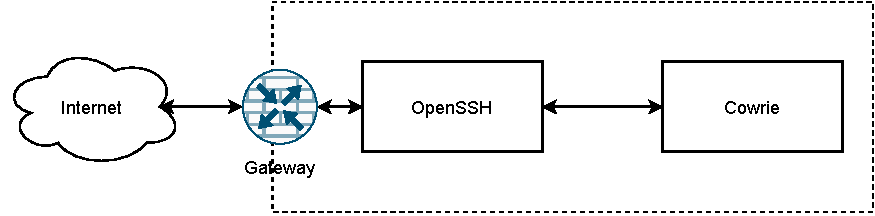
\includegraphics{figures/sshd-honeypot.pdf}
    \caption[Architecture of OpenSSH and Cowrie]{Architecture of OpenSSH and Cowrie. OpenSSH and TwistedConch have subtle differences (derived from \cite{vetterl2020})}
    \label{fig:cowrie-fix}
\end{figure}

For instance, we use the latest OpenSSH version $8.8P1$\footnote{\href{https://github.com/openssh/openssh-portable/commit/bf944e3794eff5413f2df1ef37cddf96918c6bde}{OpenSSH 8.8P1} on GitHub}.
Our implementation is based on \citet{vetterl2020} version $6.3P1$\footnote{\href{https://github.com/amv42/sshd-honeypot/commit/f58830161002baec9d3ed218e78ddb06b0d40a23}{sshd-honeypot} on GitHub}.
As mentioned beforehand, due to major differences between both versions a smooth transition is unattainable without modifications.
However, the basic idea to morph OpenSSH into an intermediary instance stays the same.
In total, to change sshd daemon to work as an intermediary includes:

\begin{itemize}
    \item A separate channel to communicate with the attacker and forward the packets to Cowrie.
    \item An authentication that permits any connection to Cowrie.
    \item Tweaking the session to write packets in the new channel.
\end{itemize}

Respectively, a detailed description of the adaption will be presented.
The easiest step is to tweak the authentication in the \verb|auth-passwd.c| to permit any session so that an incoming connection can be forwarded to Cowrie.
Originally, OpenSSH checks each session to see if the chosen authentication method returns true.
Our server has to return true for any client in the \verb|allowed_user| function to skip the authentication process.
Cowrie continues the authentication process, and communicates with the attacker.
In OpenSSH, communications are handled in channels as seen beforehand in \autoref{sec:openssh}.
Technically, the sshd daemon opens for each session a SOCKS connection to communicate with the client.
SOCKS is a network protocol to exchange packets between a server and client.
To communicate with Cowrie, the sshd daemon needs a separate channel to store the attacker's session and forward packets.
The channel is implemented in version $6.3P1$ and can be used in $8.8P1$ with minor adaptions.
In the main method when sshd is starting, the channel is created and opens a connection to the running Cowrie instance so that a new session can be forwarded.
If Cowrie is not accessible, the startup would fail.
Thus, Cowrie has to run prior to SSH.
Next, the server loop that is responsible to connect the client to the correct port has to be modified in order to put direct TCP/IP connections in our honeypot channel.
Without this adaption, no packet would be received by Cowrie.
The function \verb|server_request_direct_tcpip| handles these connections.
For instance, it checks if the TCP forwarding port for Cowrie is defined, and connects the current session to the respective port only if a communication to Cowrie is feasible.
Lastly, we have to adapt the sshd daemon to start and set up the channel.
In addition, for an easy configuration of the daemon an extension of the configuration to set the Cowrie IP address and port has been included.
After compiling our version, a brief test proofed a valid connection to the sshd daemon.

\section{Experiment 2: Avoid fingerprinting of Cowrie}

The last experiment to conclude this chapter is to test if our concept helps to disguise Cowrie and avoid fingerprinting based on a custom local string version and key exchange initialization message.
For instance, we have used \citet{vetterl2020} original $6.3P1$ sshd honeypot, as well as the newly implemented version $8.8P1$ with Cowrie version $2.3.0$.
Both versions have been tested in heiCLOUD and locally in an encapsulated environment.
All requests do not result in a bad packet length, and thus, are behaving like an original sshd daemon.
Only the older version $6.3P1$ had problems to coup with new encryption and host key algorithms.
Thus, the concept is capable of forwarding any related packet to Cowrie, and hiding the generic weakness of TwistedConch.
In \autoref{lst:log-cowrie}, Cowrie receives the connection and logs information respectively.
Currently, one downside is the connection loss that happens due to timeout restrictions.
This issue is a minor bug, and could be fixed in the future.
As a conclusion, this experiment has shown that the initial idea of hiding Cowrie in the background and directing the message through OpenSSH prevents fingerprint activities of any adversary.

\begin{figure}
    \lstinputlisting[language={}, caption={Cowrie log information.}, label={lst:log-cowrie}]{listings/cowrie.log}
\end{figure}

\section{Discussion}

Depending on the interaction-level, honeypots will always deviate from production instances.
As we have seen in the two experiments beforehand, detecting a generic weakness is doable in a respective time, as well as mitigating it.
Thus, finding and fixing weaknesses of honeypots becomes a continuous cycle.
However, this chapter also outlined the importance of the libraries that are used.
TwistedConch is the bottleneck of Cowrie and has not been updated for 10 years.
Libraries that re-implement protocols have to be always up-to-date.
As a conclusion, such libraries should be chosen carefully to avoid any bugs which leaves harmful information to attackers.

\begin{figure}
    \centering
    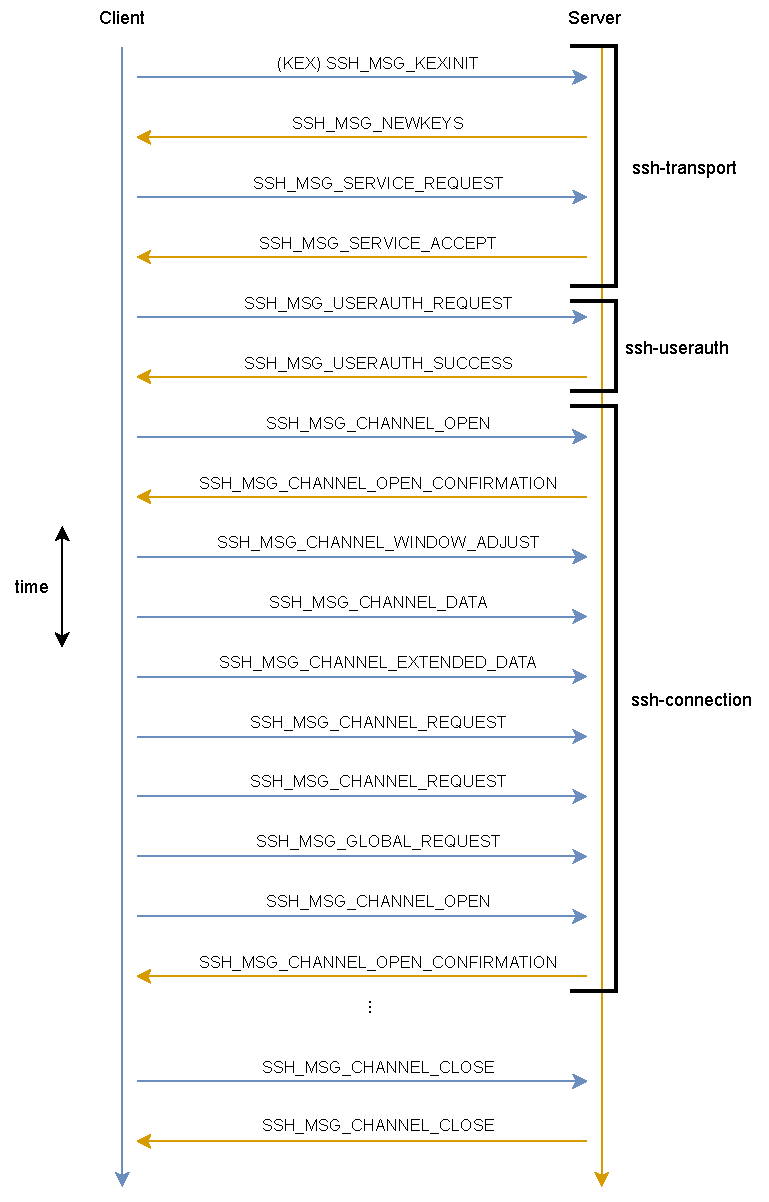
\includegraphics{figures/ssh-flow-diagram.pdf}
    \caption[OpenSSH sample session flow diagram]{OpenSSH sample session flow diagram (derived from \cite{openssh2007}). In addition, on the right side indicates the layers that are responsible for handling the messages.}
    \label{fig:openssh-flow-diagram}
\end{figure}